
\documentclass[letterpaper, 10 pt, conference]{ieeeconf}  % Comment this line out if you need a4paper
\usepackage{graphicx}



%\documentclass[a4paper, 10pt, conference]{ieeeconf}      % Use this line for a4 paper

\IEEEoverridecommandlockouts                              % This command is only needed if 
                                                          % you want to use the \thanks command

\overrideIEEEmargins                                      % Needed to meet printer requirements.

% See the \addtolength command later in the file to balance the column lengths
% on the last page of the document

% The following packages can be found on http:\\www.ctan.org
%\usepackage{graphics} % for pdf, bitmapped graphics files
%\usepackage{epsfig} % for postscript graphics files
%\usepackage{mathptmx} % assumes new font selection scheme installed
%\usepackage{times} % assumes new font selection scheme installed
%\usepackage{amsmath} % assumes amsmath package installed
%\usepackage{amssymb}  % assumes amsmath package installed
\usepackage{cite}
\usepackage{mathtools}
\usepackage{cleveref}
\graphicspath{{./pictures/}}

\title{\LARGE \bf
Magnetic Hammer Actuation for Tissue Penetration using Millirobots}


\author{Julien Leclerc, Ashwin Ramakrishnan, Nikolaos V. Tsekos, and Aaron T. Becker % <-this % stops a space
\thanks{This work was supported by the National Science Foundation, Grant No. 1646566. }% <-this % stops a space
\thanks{Authors are with the Dept. of Electrical and Computer
Engineering, University of Houston, Houston, TX 70004, USA
        {\tt\small jleclerc@uh.edu}}%
%\thanks{$^{2}$Bernard D. Researcheris with the Department of Electrical Engineering, Wright State University,
%       Dayton, OH 45435, USA
%      {\tt\small b.d.researcher@ieee.org}}%
}


\begin{document}



\maketitle
\thispagestyle{empty}
\pagestyle{empty}


%%%%%%%%%%%%%%%%%%%%%%%%%%%%%%%%%%%%%%%%%%%%%%%%%%%%%%%%%%%%%%%%%%%%%%%%%%%%%%%%
\begin{abstract}

Untethered magnetic navigation of millirobots within a human body using an MRI scanner is a promising technology for minimally invasive surgery or drug delivery.
Because MRI scanners have a large static magnetic field, they cannot generate torque on magnetic millirobots and must instead use gradient-based pulling.
 However, gradient values are too small to produce forces large enough to penetrate tissue. 
 This paper presents a method to produce large pulsed forces on millirobots. 
 A ferromagnetic sphere is placed inside a hollow robot body and can move back and forth. 
 This movement is created by alternating the magnetic gradient direction. 
 On the posterior side, a spring allows the sphere to change direction smoothly. 
 On the anterior side, a hard rod creates a surface for the sphere to impact. 
 This impact results in a large pulsed force. 
 This paper begins with modeling and simulating this system. 
 Next, a control strategy is presented and experimentally tested.
  Finally, preliminary tests inside a clinical MRI scanner demonstrate the potential of this actuation system. 

\end{abstract}


%%%%%%%%%%%%%%%%%%%%%%%%%%%%%%%%%%%%%%%%%%%%%%%%%%%%%%%%%%%%%%%%%%%%%%%%%%%%%%%%
\section{INTRODUCTION}

The navigation of millimeter-scale robots through the passageways of bodies is currently being studied as a method to perform highly localized drug delivery or perform minimally invasive surgery \cite{7067029,702,mi2020295}. Untethered navigation can be achieved by placing a ferromagnetic piece inside the robot and producing a controlled magnetic field around a patient. Propulsion and steering of millirobots can be accomplished by either moving a permanent magnet assembly around a patient \cite{taylor} or by controlling the current inside electromagnets \cite{MRM21638}. The latest solution is often realized with an MRI scanner which already includes several electromagnets. In an MRI, the background field magnetizes the ferrous components of the robot, and the gradient coils generate the magnetic gradient necessary to produce forces. 
The MRI scanner can be used simultaneously to provide real-time imaging of the operating area as well as positioning of the robot.\par
The force generated on the millirobots is proportional to the field gradient strength. 
Commercial MRI scanners produce gradients in the range of 20 to 40 mT/m. 
These gradients are sufficient to maneuver milli-robots inside fluid-filled regions of the body, such as vessels, \cite{martel2007automatic} but insufficient for tissue penetration that requires larger forces \cite{7139341}; tissue penetration is required for many procedures, including brachytherapy and micro-biopsy.
This paper presents a method, denoted  \emph{magnetic hammer actuation}, that can generate large pulsed forces for tissue penetration. 
The magnetic hammer is a system embedded into the millirobot. 
The millirobot has a tubular structure in which a ferromagnetic sphere can move back and forth.
 This movement is produced by alternately changing the gradient direction. 
 On the posterior side of the millirobot, a spring allows the sphere to change direction smoothly. 
 On the anterior side, a hard rod creates a surface for the sphere to impact, the \emph{impact plate}.
  This impact results in large pulsed forces that enable penetrating body tissues progressively.
A magnetic test bench has been developed to make experimental tests more practical and less expensive.
 It includes coils, sensors, power electronics, and a real-time controller.\par

\begin{figure}
  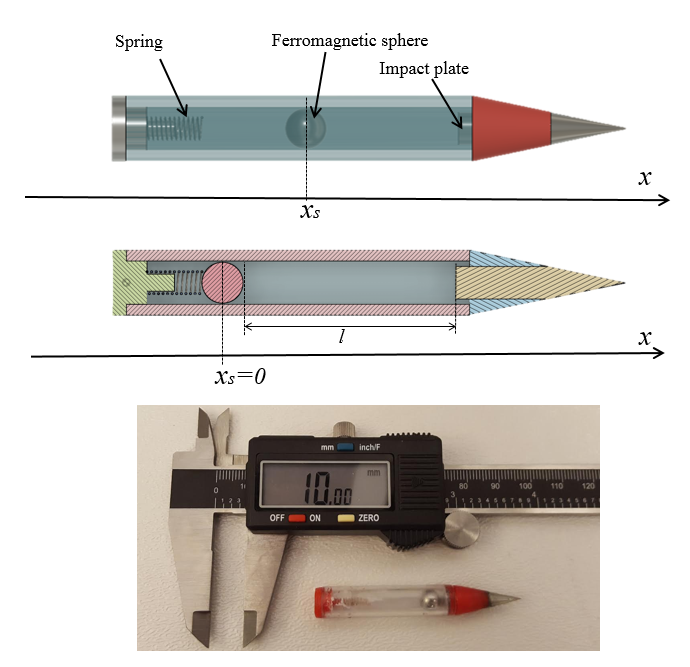
\includegraphics[width=\linewidth]{figure1-2.png}
  \caption{Schematic representation of a millirobot actuated by a magnetic hammer (top), hardware prototype (bottom).}
  \label{millirobot}
  \vspace{-2em}
\end{figure}

The paper is organized as follows: first, the system is mathematically modeled, and its behavior is studied in \cref{theoretical}. Secondly, parameters for the model are experimentally measured (see \cref{cor_det}). Different materials for the impact plate are compared. Thirdly, the magnetic test bench is described and the test of a magnetic hammer is presented (see \cref{experiment}). Results are compared to the mathematical model. Next, preliminary results from an open-loop test performed in a clinical MRI scanner are presented in \cref{MRI_tests}. The last section (\cref{conclusion}) is a conclusion of this study.


\section{Theoretical study}
\label{theoretical}
\subsection{Mechanical modelization}
The motion of the sphere between two consecutive impacts can be divided into two  phases, based on the forces that act on it. The magnetic gradient force $F_{mag}$ and friction force $F_{friction}$ act on the sphere during its motion along the free length of the tube, $L$ (See Fig. \ref{FBD} (i),(iii)). When the spring is compressed, its reaction force $F_{spring}$ acts on the ball as well (See Fig. \ref{FBD} (ii)). The directions of $F_{mag}$ and $F_{friction}$  change depending on the direction of motion of the sphere. 
\begin{figure}
	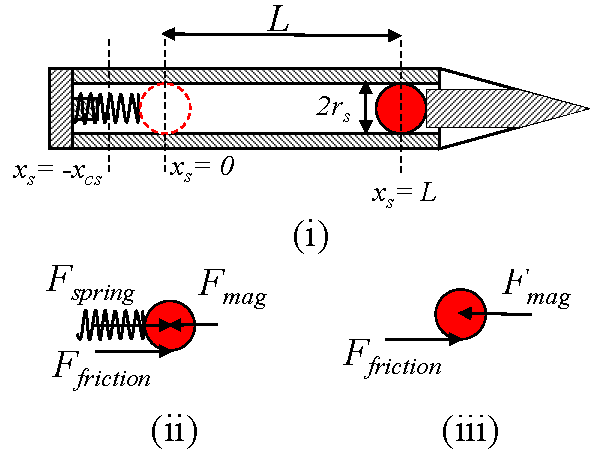
\includegraphics[width=\linewidth]{FBD_R1.pdf}
	\caption{(i) Free length of sphere travel, $L$; (ii) Free body diagram of sphere when spring is compressed, (iii) when spring is not compressed}
	\label{FBD}
\end{figure}
Inside the homogeneous region of an MRI scanner, the magnitude of $F_{mag}$ is constant \cite{CMR:CMR20163}. The same has been assumed for developing analytical and numerical models in this paper. The formula for calculating $F_{mag}$ is presented in section II-B. Friction is considered to be negligible, but the assumption will be relaxed in later sections. The spring force is straightforward, and is given by
\begin{equation}
F_{\text{spring}}=k x,
\label{spring_force}
\end{equation}
where $x$ is the compression length, and $k$ is the spring constant. To maximize the average impact velocity over an arbitrary $n$ number of contacts, the input magnetic gradient should always be in the same direction as the motion of the sphere. This is equivalent to a perfectly closed-loop system where the gradient signal switches direction when the sphere switches direction.

An analytical model was developed by solving the system ODE to predict the impact velocity for each impact, given a set of input parameters. The sphere-impact plate system is assumed to have a coefficient of restitution, $e$. This model assumes that the robot capsule does not move. For all values of $e$, the impact velocity initially increases and ultimately saturates, reaching a resonant value. This happens when the energy lost by the sphere during impact equals the energy gained by it during the rest of the cycle. A higher $e$ results in a higher impact velocity.  Figure \ref{CLinput} shows a sample closed-loop pulsed magnetic gradient input for 50 impacts. The frequency initially varies until it settles to a constant value at resonance. An analytical formula was derived to predict the resonant impact velocity, for a given set of input parameters. This is given by \cref{Resonant_CLvelocity}.
%\begin{figure}
%	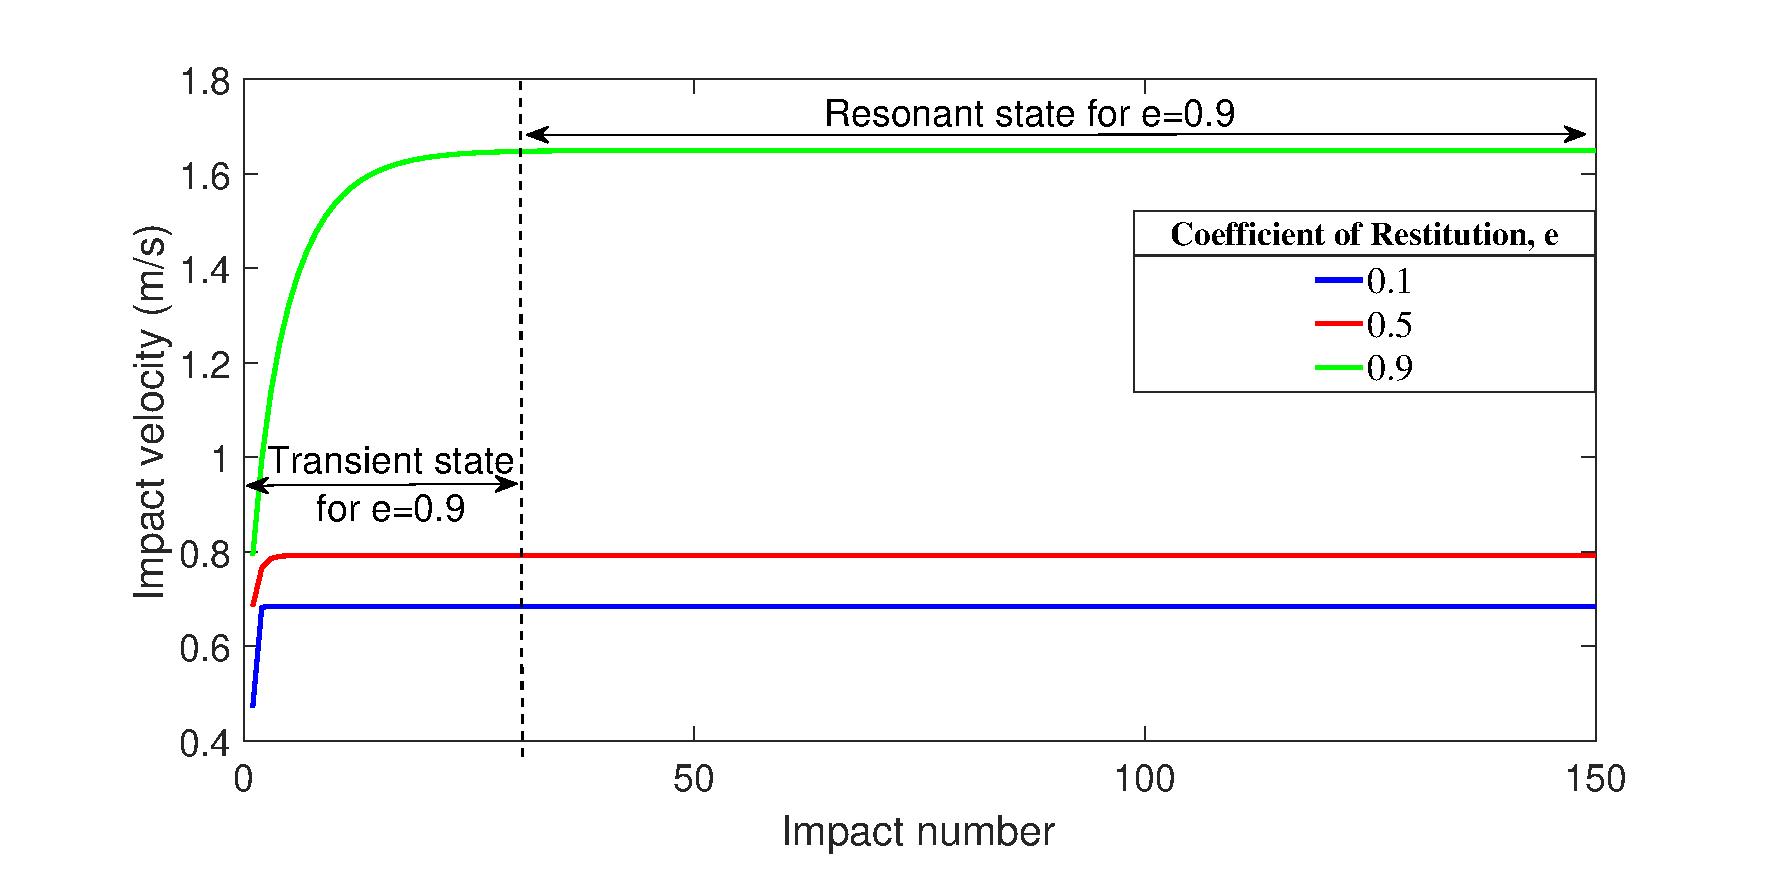
\includegraphics[width=\linewidth]{Closedloop_Impact_velocity.eps}
%	\caption{Closed loop impact velocity for 150 impacts; $k$ = 50 N/m; $e$ = 0.9; $F_{mag}$ = 1.5e-3 N; $L$ = 0.03 m; $m_s$ = 5.58e-4 kg; $r_s$ = 2.5 mm.}
%	\label{Closedloop_Impact_velocity}
%	
%\end{figure}
\begin{equation}
\resizebox{\linewidth}{!}
{$
	v_{\text{res}}=\frac{2 \sqrt{\frac{F_{\text{mag}} \left(\left(e^2+1\right) F_{\text{mag}}+\left(e^2-1\right) (-k) L+\sqrt{\left(2-2 e^4\right) k L F_{\text{mag}}+\left(1+e^2\right)^2 F_{\text{mag}}^2}\right)}{k m_s}}}{1-e^2}
	$}
\label{Resonant_CLvelocity}
\end{equation}
In the above equation, $m_s$ is the mass of the sphere in kgs. The radius of the ball $r_s$ indirectly influences the impact velocity through $F_{mag}$ and $m_s$, both of which depend on the volume of the sphere. The variation of $v_{res}$ with changes in $L,e,k,m_s,r_s,F_{mag}$ were plotted and they were all found to be monotonic functions with no critical points. In \cref{Resonant_CLvelocity}, $v_{res}$ tends towards infinity as $e$ tends to 1. In this case there is no loss of energy during collision and hence, the impact velocity indefinitely increases with subsequent impacts. Further, the time between impacts at resonance $t_{res}$, is a constant value and is given by \cref{tres6}.

\begin{equation}
t_{res}=t_{pos,1}+t_{pos,2}+t_{ant,1}+t_{ant,2}
\label{tres6}
\end{equation}	
\begin{equation}
t_{pos,1}=\frac{\sqrt{e^2 v_{\text{res}}^2+\frac{2 L F_{\text{mag}}}{m_s}}-e v_{\text{res}}}{\frac{F_{\text{mag}}}{m_s}}
\label{tres1}
\end{equation}
\begin{equation}
t_{pos,2}=\frac{\pi -\tan ^{-1}\left(\frac{k \sqrt{e^2 v_{\text{res}}^2+\frac{2 L F_{\text{mag}}}{m_s}}}{\omega  F_{\text{mag}}}\right)}{\omega } ; \text{$\omega $ = }
\sqrt{\frac{k}{m_s}}
\label{tres2}
\end{equation}
\begin{equation}
t_{ant,1}=\frac{\cos ^{-1}\left(\frac{F_{\text{mag}}}{F_{\text{mag}}+k x_{cs}}\right)}{\omega }
\label{tres3}
\end{equation}
\begin{equation}
t_{ant,2}=\frac{v_{\text{res}}-\sqrt{v_{\text{res}}^2-\frac{2 L F_{\text{mag}}}{m_s}}}{\frac{F_{\text{mag}}}{m_s}}
\label{tres4}
\end{equation}
\begin{equation}
x_{cs}=\frac{\sqrt{e^2 k m_s v_{\text{res}}^2+2 k L F_{\text{mag}}+F_{\text{mag}}^2}+F_{\text{mag}}}{k}
\label{tres5}
\end{equation}


In the above equations, $x_{cs}$ is the maximum compression distance of the spring (See Fig. \ref{FBD} (i)), and $\omega$ represents the natural frequency of the spring-mass system. The value of $x_{cs}$ can be used to select an appropriate free length for the spring, to ensure that it does not bottom out during compression. The values $t_{pos,1}$, $t_{pos,2}$, $t_{ant,1}$ and $t_{ant,2}$ represent the time for the ball to move from $x_S =$ (i) $L$ to 0, (ii) 0 to $-x_{cs}$, (iii) $-x_{cs}$ to 0, and (iv) 0 to $L$ respectively, in a perfectly closed-loop system with optimal gradient switching.



\begin{figure}
	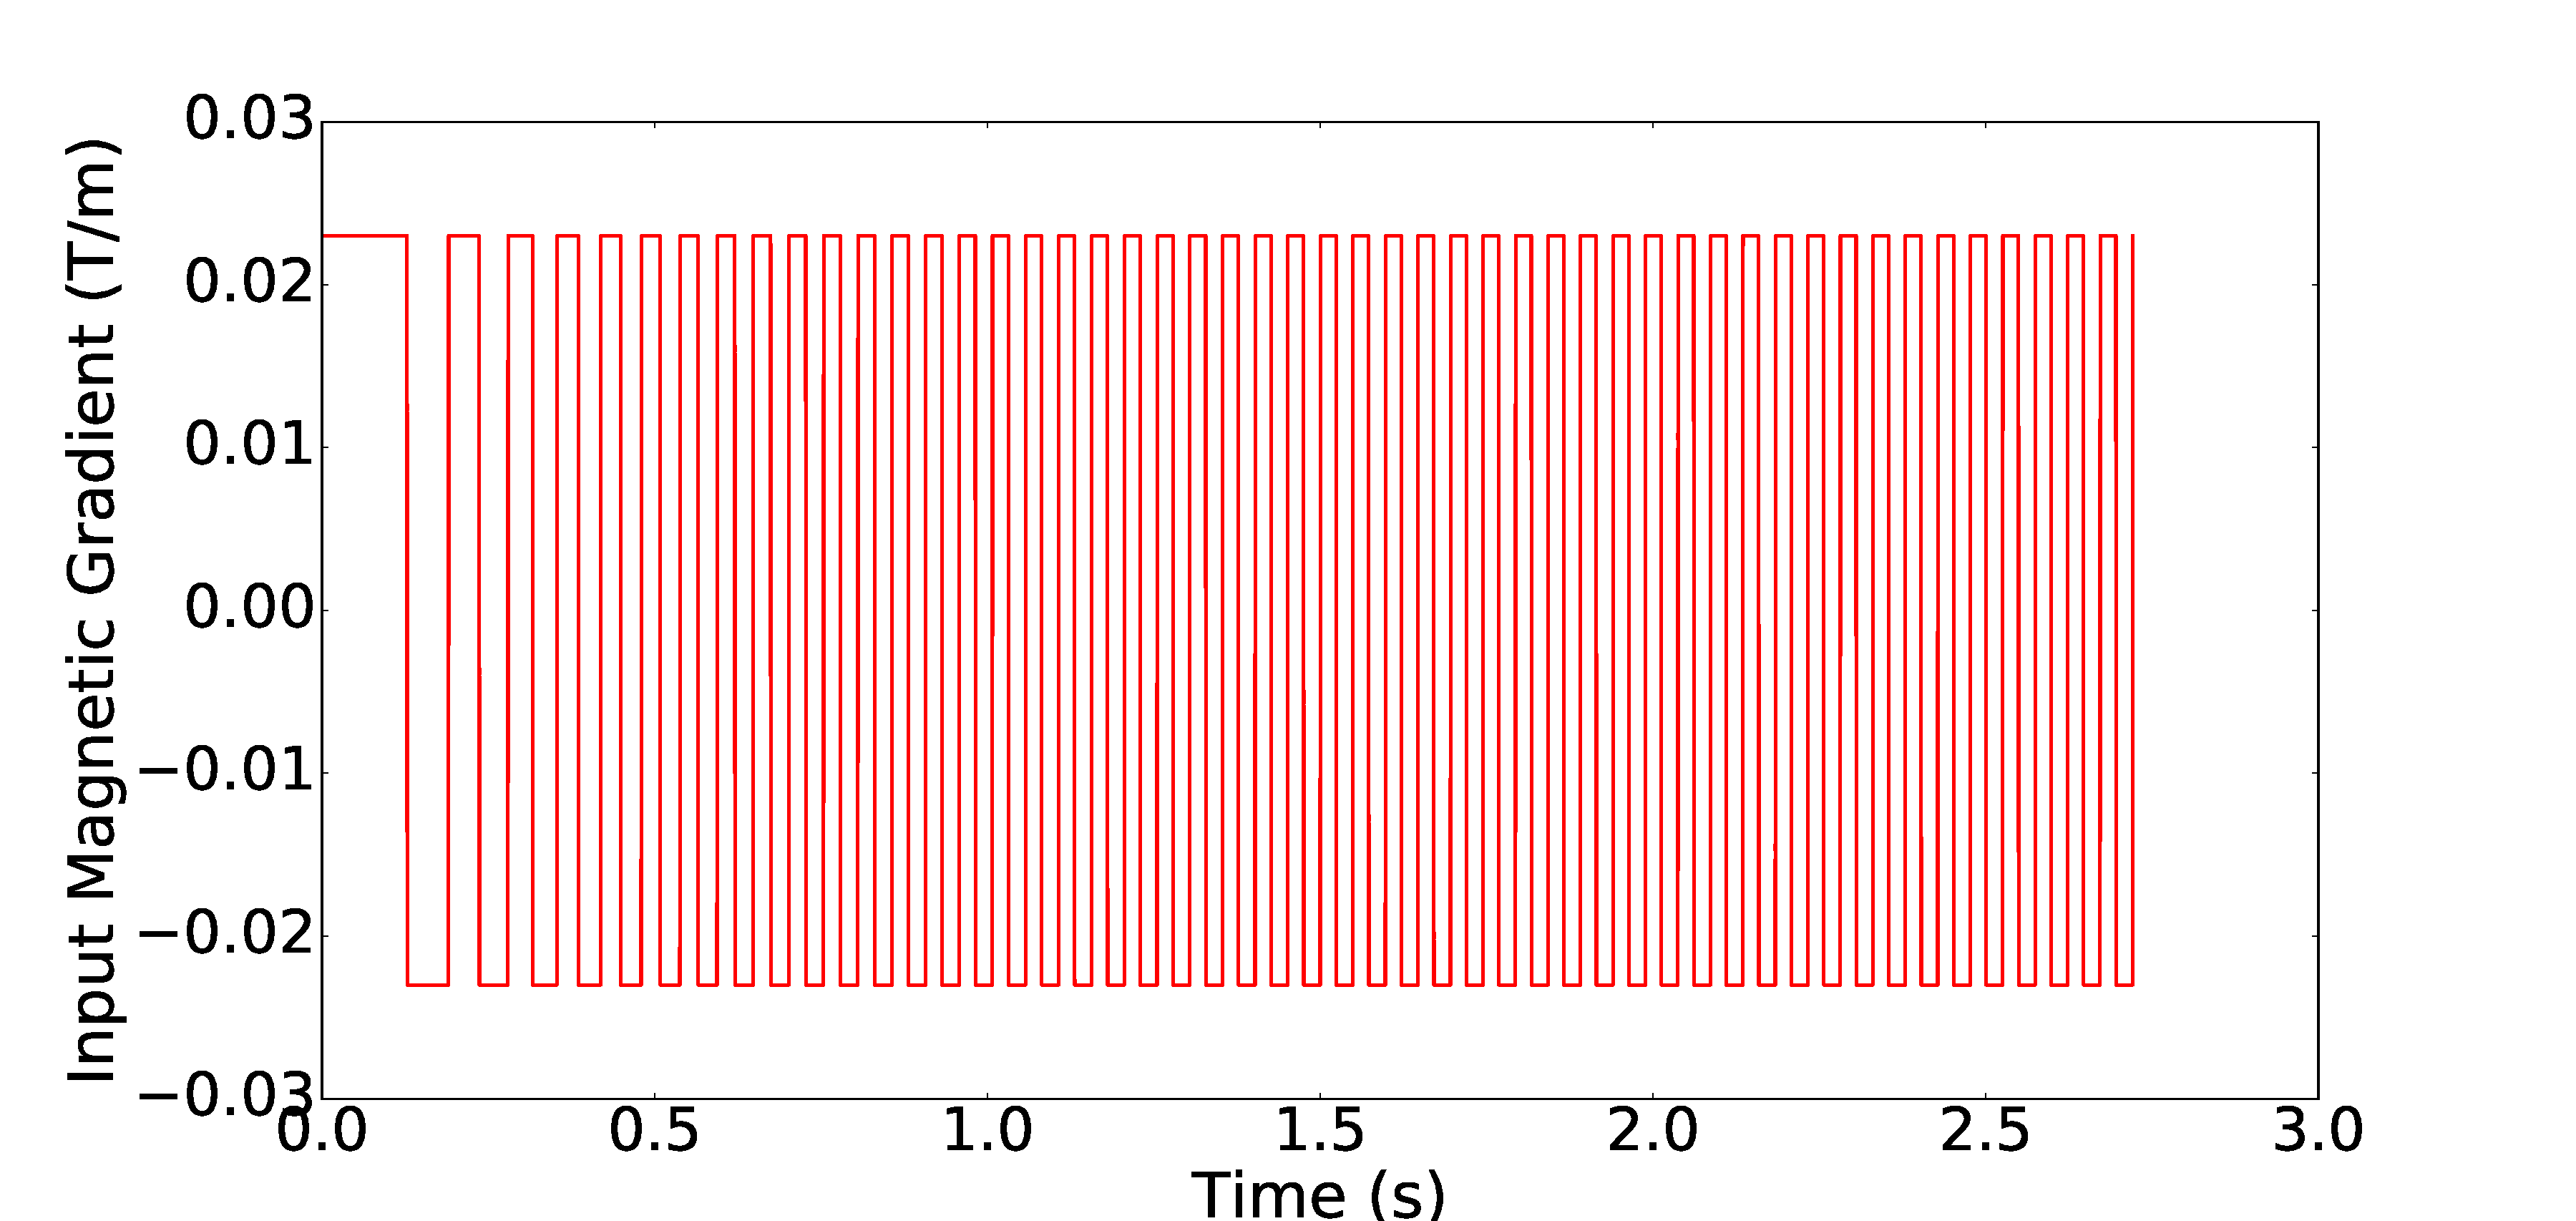
\includegraphics[width=\linewidth]{CLinput.pdf}
	\caption{Closed loop input gradient for 50 impacts; $k$ = 50 N/m; $e$ = 0.9; $F_{mag}$ = 1.5e-3 N; $L$ = 0.03 m; $m_s$ = 5.58e-4 kg; $r_s$ = 0.0025 m.}
	\label{CLinput}
	
\end{figure}

\subsection{Magnetic field calculation}
\label{magfield}
The magnetic field generated by an MRI scanner can be separated into two components. The first is a constant and strong magnetic field $B_0$ along the z-axis. This field is used to align the magnetic moments of the protons. Commercial MRI scanners have $B_0$ typically ranging from 1.5 to 3 T. The second component of the field is the magnetic gradient. It is used to encode the MRI signal spatially. The flux density $\mathbf{G}$ produced by the gradient coils is added to $\mathbf{B_0}$ and linearly varies with position. A computer controls this value.\par
The modelization of the field inside the uniformity sphere of an MRI scanner is straightforward. $\mathbf{G}$ is directly proportional to the current inside the gradient coils. 

\begin{equation}
\mathbf{B}=\mathbf{B_0}+\mathbf{G},~~~
\mathbf{B_0}=\begin{bmatrix}
0\\ 
0\\ 
B_0
\end{bmatrix},~
\mathbf{G}=\begin{bmatrix}
k_x I_x\\ 
k_y I_y\\ 
k_z I_z
\end{bmatrix}
\label{magfield}
\end{equation}

where $k_x$, $k_y$ and $k_z$ are the coil constants (T/A) and $I_x$, $I_y$ and $I_z$ are the electrical current values.\par

The flux density is more complicated to calculate outside of the uniformity sphere. The same problem is present in our desktop experiment because the flux density and gradient are not constant. To calculate forces accurately, it is necessary to compute the magnetic field precisely. A semi analytical method was used to calculate the field produced in all space by a solenoid assembly. It was tested on our desktop experiment.\par
According to \cite{simpson2001simple}, the magnetic flux density produced by a current loop in all space can be calculated using equations \cref{Bz1loop,Bteta1loop,delta,beta,single_loop_geometry}. $E(k)$ and $K(k)$ are the complete elliptical integrals of first and second kind respectively.
\begin{equation}
B_z=\frac{\mu _0I}{2\pi\delta ^{2}\beta  }\left [ \left ( a^2-\rho ^2-z^2 \right )(E(k^2)+\delta ^2K(k^2)) \right ] 
\label{Bz1loop}
\end{equation}
\begin{equation}
B_\theta=\frac{\mu _0 I \cdot z}{2\pi\delta ^{2}\beta\rho   }\left [ \left ( a^2-\rho ^2-z^2 \right )(E(k^2)-\delta ^2K(k^2)) \right ]
\label{Bteta1loop}
\end{equation}
\begin{equation}
\delta =\sqrt{a^2+R_m^2+Z_m^2-2aR_m}
\label{delta}
\end{equation}
\begin{equation}
\beta =\sqrt{a^2+R_m^2+Z_m^2+2aR_m}
\label{beta}
\end{equation}

\begin{figure}
  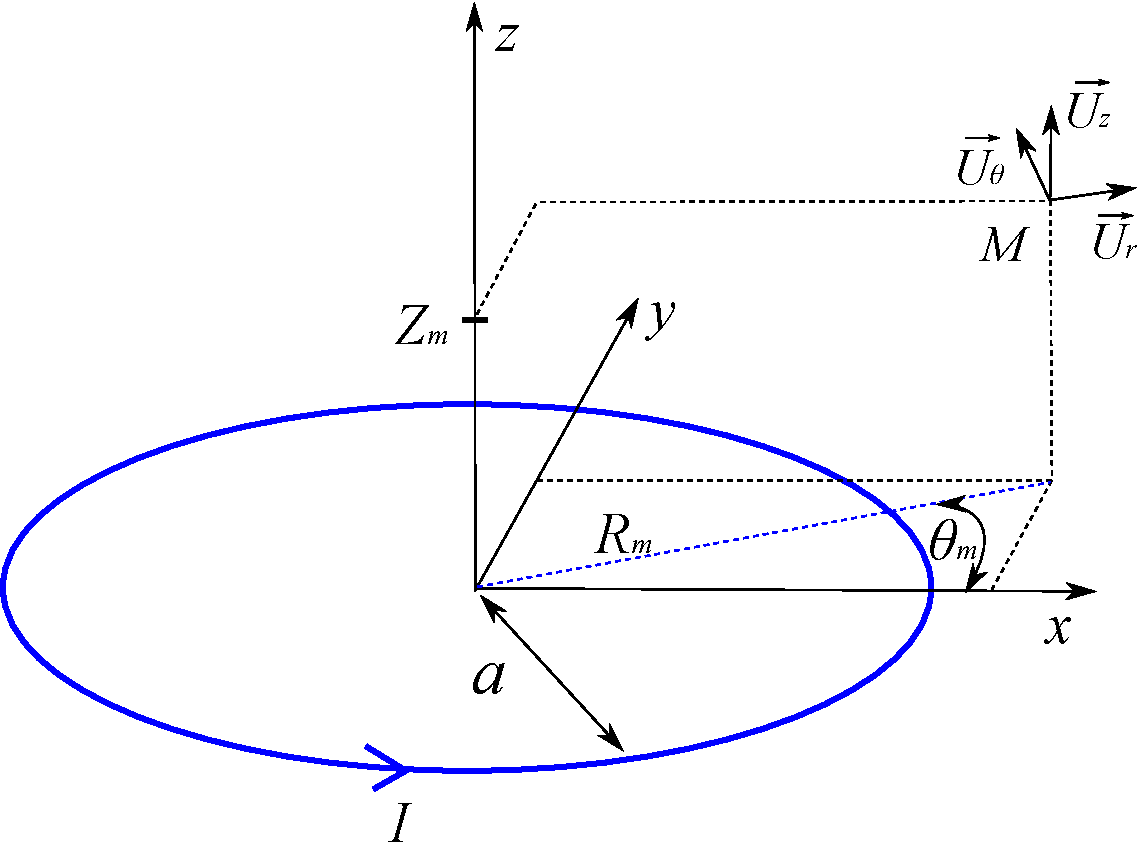
\includegraphics[width=\linewidth]{single_loop.pdf}
  \caption{Geometry and variables used in equation \cref{Bz1loop,Bteta1loop,delta,beta}}
  \label{single_loop_geometry}
\end{figure}

The cross-section $S$ of any solenoid can be divided into infinitesimal sections $dS$. Each $dS$ is subjected to a current $dI=JdS$. This current $dI$ forms an infinitesimal loop, and the field it produces can be calculated using \cref{Bz1loop,Bteta1loop,delta,beta}. By integrating this equation over the solenoid cross-section, one can obtain the value of the flux density generated by the solenoid.\par
The flux density must be calculated for each solenoid. The total flux density is the vectorial sum of the flux density produced by each solenoid. The results obtained via this semi analytical method is compared to the solution obtained via finite element calculations with the software FEMM \cite{femm} (see fig. \ref{Femm_matlab_comparison}). The results are identical. The semi-analytical method is faster to compute for this model. Indeed, the magnetic field only needs to be calculated at the sphere position. The semi-analytical method can calculate the magnetic field at one point only whereas, finite elements methods must compute the magnetic field in the full domain.

\begin{figure}
  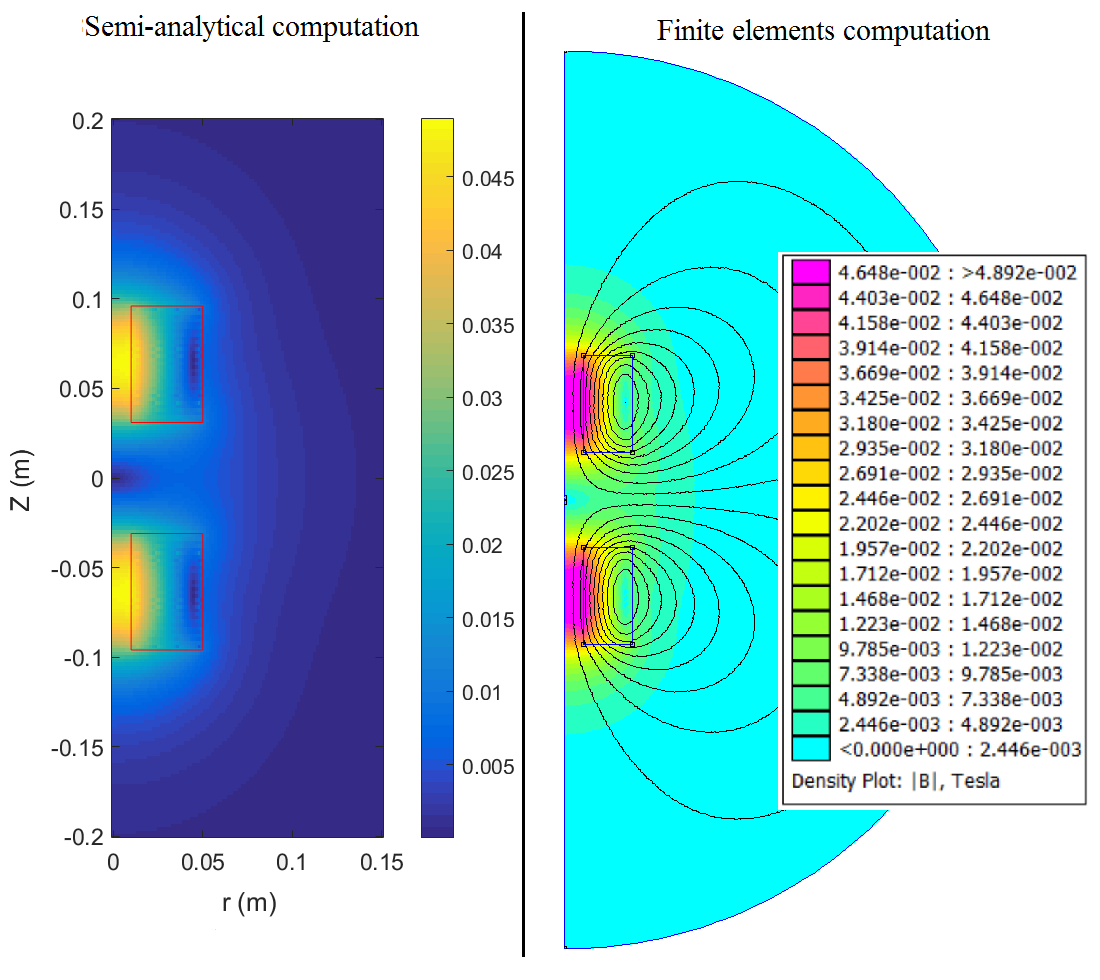
\includegraphics[width=\linewidth]{Femm_matlab_comparison.png}
  \caption{Comparison between the flux density computed with the semi-analytical method with {\sc Matlab} and the flux density computed via a finite element method with FEMM.}
  \label{Femm_matlab_comparison}
\end{figure}

\subsection{Magnetic force calculation}
\label{magforce}

This section calculates the force applied by the magnetic field to the sphere.\par
The ferromagnetic sphere is small compared to the coil system and can be considered as a infinitely small magnetic moment $\mathbf{m}$. Assuming a constant material magnetization $\mathbf{M}$, one can calculate $\mathbf{m}$ from \cref{mag}.

\begin{figure}
	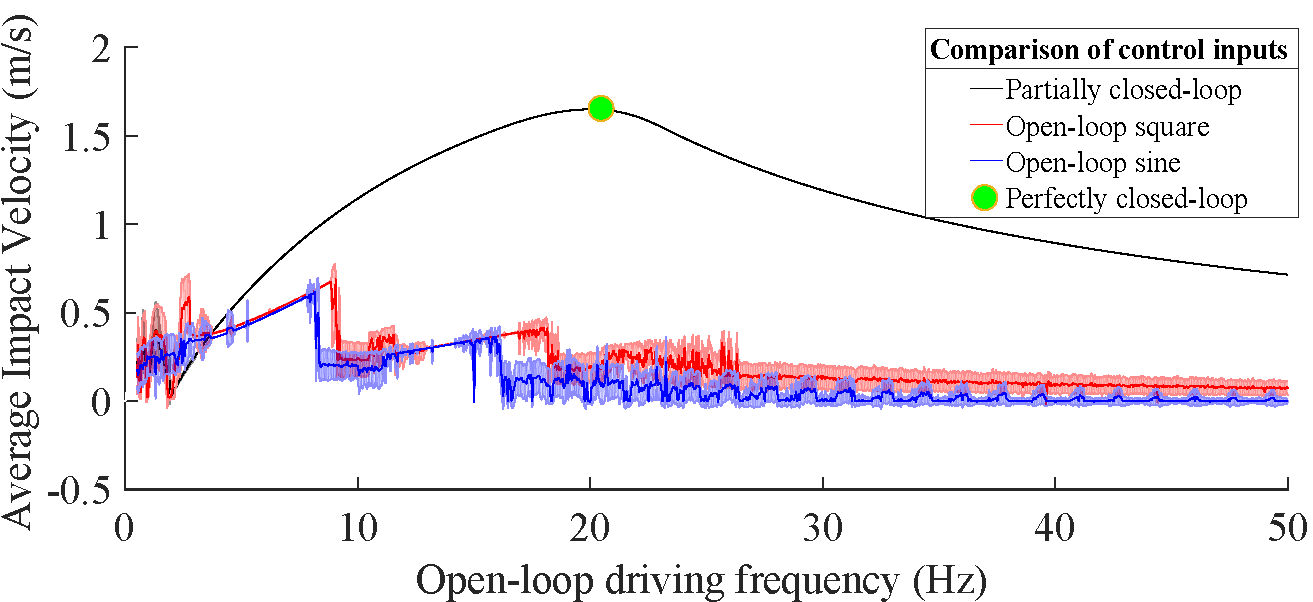
\includegraphics[width=\linewidth]{ComparisonOfControlInputs.pdf}
	\caption[Comparison of impact velocities from three control inputs]{Comparison of average impact velocities between impacts 100 and 1100 for three different control inputs: Open-loop vs. Partially closed-loop vs. Ideally closed-loop}
	\label{CLvsOL}
\end{figure}

 $V$ is the volume of the sphere.
The ferromagnetic sphere is magnetized by the externally applied field $\mathbf{H}_{app}=\mathbf{B}_{app}/\mu_0$. Ferromagnetic materials create a demagnetizing field $\mathbf{H}_d$ when subjected to an external field. The actual field $\mathbf{H}$ seen by the sphere is the sum of $\mathbf{H}_{app}$ and $\mathbf{H}_d$. This effect must be taken into account to calculate the magnetization accurately. $\mathbf{H}_d$ is related to $\mathbf{H}_{app}$ by \cref{hd}. The demagnetization factor $N$ for a sphere is -1/3. Its magnetization can be calculated using \cref{mag2}.
Once the magnetic moment $\mathbf{m}$ is obtained, the force on the sphere can be calculated using \cref{force}.

\begin{align}
\mathbf{m}&=\mathbf{M}.V \label{mag}\\
\mathbf{H}_d&=N.\mathbf{H}_{app}\label{hd}\\
\mathbf{M}&=\frac{\mathbf{H}_{app}\left ( \mu_r-1  \right )}{2.N.\mu_r-1} \label{mag2}\\
\mathbf{F}&=\mathbf{\nabla}(\mathbf{m}.\mathbf{B}) \label{force}
\end{align}

\subsection{Simulation results}

\subsubsection{Perfectly closed loop vs. open loop system}
\label{clol}

A numerical model was used to simulate the system dynamics for different input gradients. Average impact velocities over impacts 100 to 200 were compared for a perfectly closed loop pulsed input, and open loop inputs with sinusoidal and square profiles. As seen in figure \ref{CLvsOL}, closed loop control produces approximately three times greater average impact velocity as compared to open loop sinusoidal and square waves, over all frequencies. As with the analytical model in section II-A, the simulation assumes that the robot capsule does not translate along its axis. While the absolute values of impact velocity and force will be different when the capsule is free to move, the closed-loop input can still be expected to produce higher forces than open-loop inputs. Further, for a given open-loop frequency, the variation of impact velocity over multiple contacts was found to be random for both square and sinusoidal inputs. It is not possible to reach the resonant state using a constant frequency input of any form. For a given set of input parameters, there exists only one path, or control input, that enables the system to reach a resonant state. 
\begin{figure}
	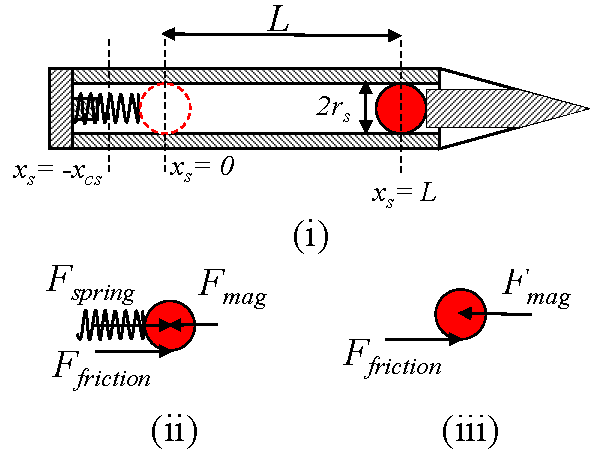
\includegraphics[width=\linewidth]{Tswitchcases.pdf}
	\caption{Six domains for spring-end switching time; green and red represent $F_{mag}$ towards anterior and posterior respectively. Direction of colored arrow represents direction of ball motion.}
	\label{Tswitch}
\end{figure}


\subsubsection{Partially closed loop system}

To implement a perfectly closed loop system, sensing is required at both the spring and impact ends. While sensing at the impact end can be done using a microphone sensor (see section III-B), it is harder to detect sphere reversal at the spring end. For experiments of the magnetic hammer on our test bench, a partially closed-loop system was implemented with only impact end sensing using a microphone. The sensor detected each impact and triggered a reversal in the direction of the gradient force. The switching time $t_s$ at the spring end was manually set at different values. There are six regimes for $t_s$, for a given set of geometric and material properties as shown in \cref{Tswitch}. In \cref{Tswitch}(i), the initial velocity $v_{0^+}$ and $t_s$ are low enough that the sphere reverses direction before reaching the spring. In this case, $v_{0^+} < 2aL$, where $a=F_{mag}/m_s$. Fig. \ref{Tswitch}(ii) represents the case when $v_{0^+}$ is high enough that spring compression is unavoidable even for $t_s = 0$. In \cref{Tswitch}(iii), the signal switch happens after spring compression starts but before it bottoms out. Fig. \ref{Tswitch}(iv) represents perfect closed loop switching. In \cref{Tswitch}(v), the signal is switched after maximum compression, but before the sphere reaches $x_s=0$. Fig. \ref{Tswitch}(vi) represents switching after spring rebound and before the next impact. There is also a possible seventh case where the switching happens after one entire impact cycle. This case is not relevant and serves more as an upper limit of practical $t_s$ values. 

Simulations were done for the partially closed loop system to identify effects of different $t_s$ values. The variation of time between impacts $\Delta t_{imp}$, with changes in $t_s$ and initial velocity $v_{0^+}$ have been plotted. Fig. \ref{delTvsTs} shows $\Delta t_{imp}$ as a function of $t_s$. For $v_{0^+}=0.15\text{ m/s}$, there is a linear increase in $\Delta t_{imp}$ till $t_s$ reaches a critical point. This linear region represents the case shown in \cref{Tswitch}(i). Beyond this, $\Delta t_{imp}$ decreases with increasing $t_s$ (\cref{Tswitch}(ii),(iii)), until the latter reaches its perfectly closed-loop value. At this point $\Delta t_{imp}$ reaches a minimum value (\cref{Tswitch}(iv)). As $t_s$ increases beyond this, the $\Delta t_{imp}$ keeps increasing (\cref{Tswitch}(v),(vi)), until it saturates because the signal is switched after the duration of the entire impact cycle. The linear range does not exist for higher values of $v_{0^+}$. Using these models, we intend to design a control law that will help push $t_s$ values closer to perfectly closed-loop values for subsequent impacts.


\begin{figure}
	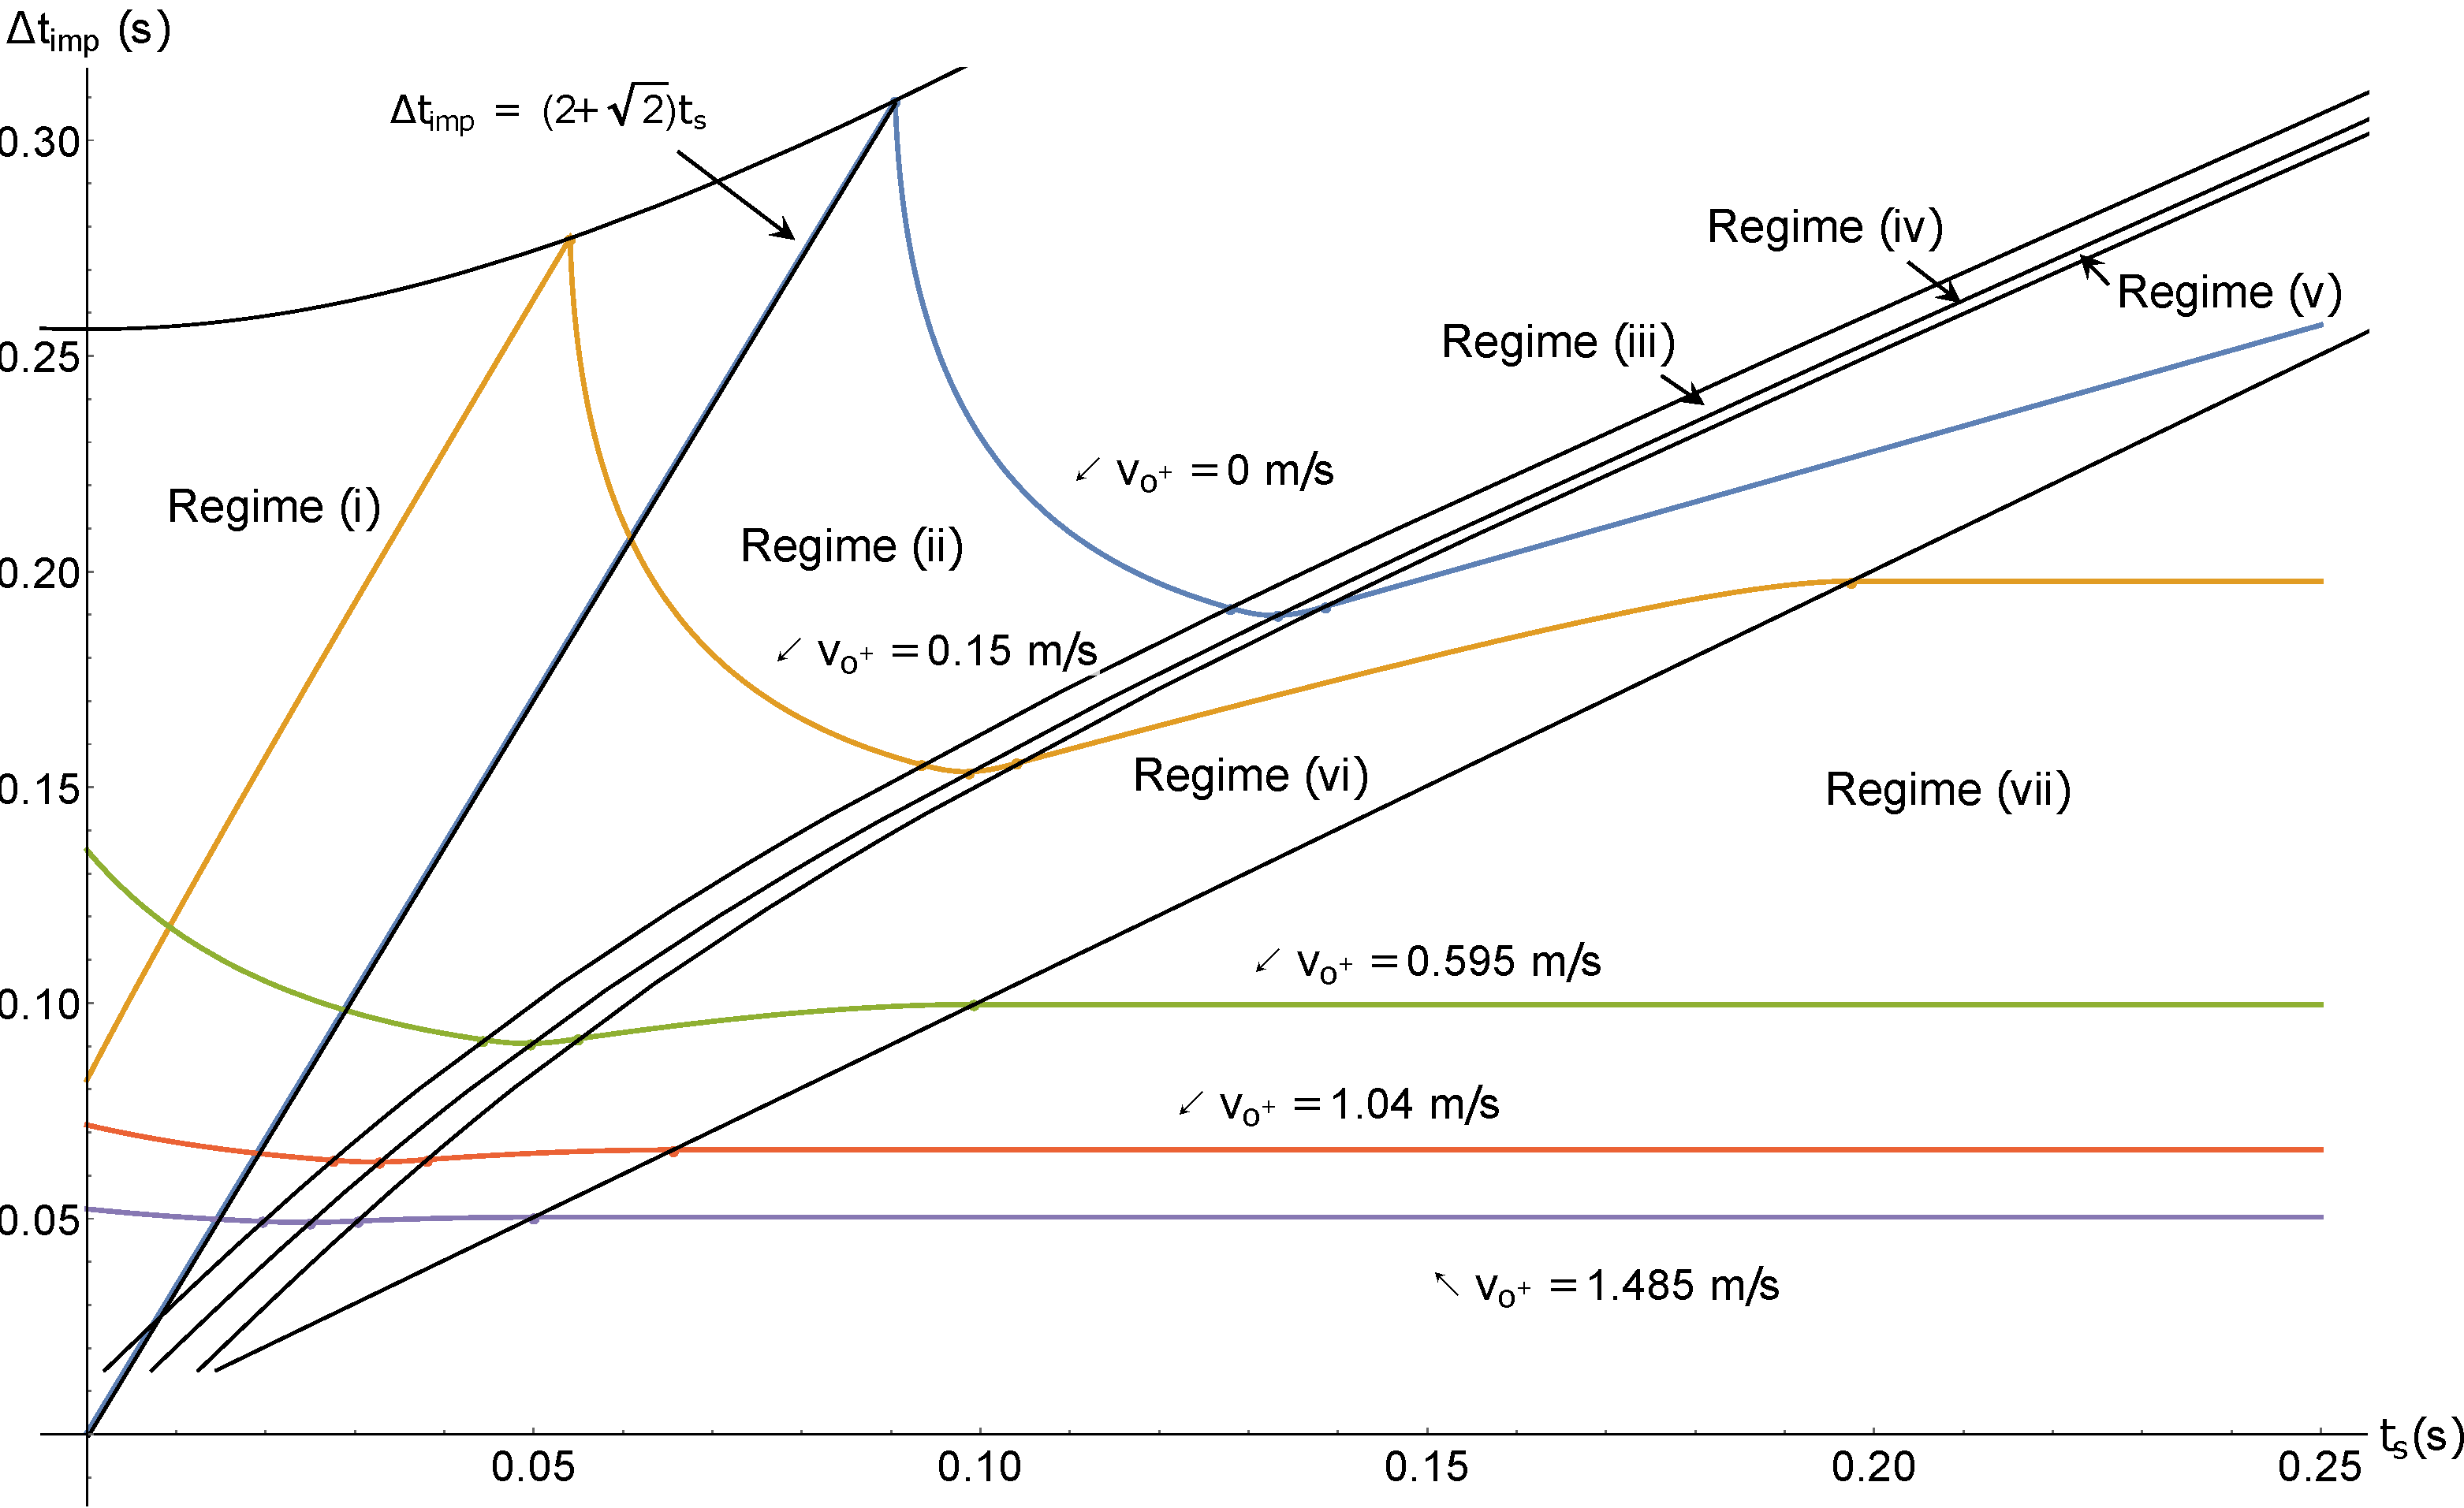
\includegraphics[width=\linewidth]{deltVsts_differentVop.pdf}
	\caption[Variation of time between impacts with switching time for partially closed-loop control]{Plot of $\Delta t$ vs. $t_s$ for different values of $v_{o^+}$.}
	\label{delTvsTs}
\end{figure}
\begin{figure}
	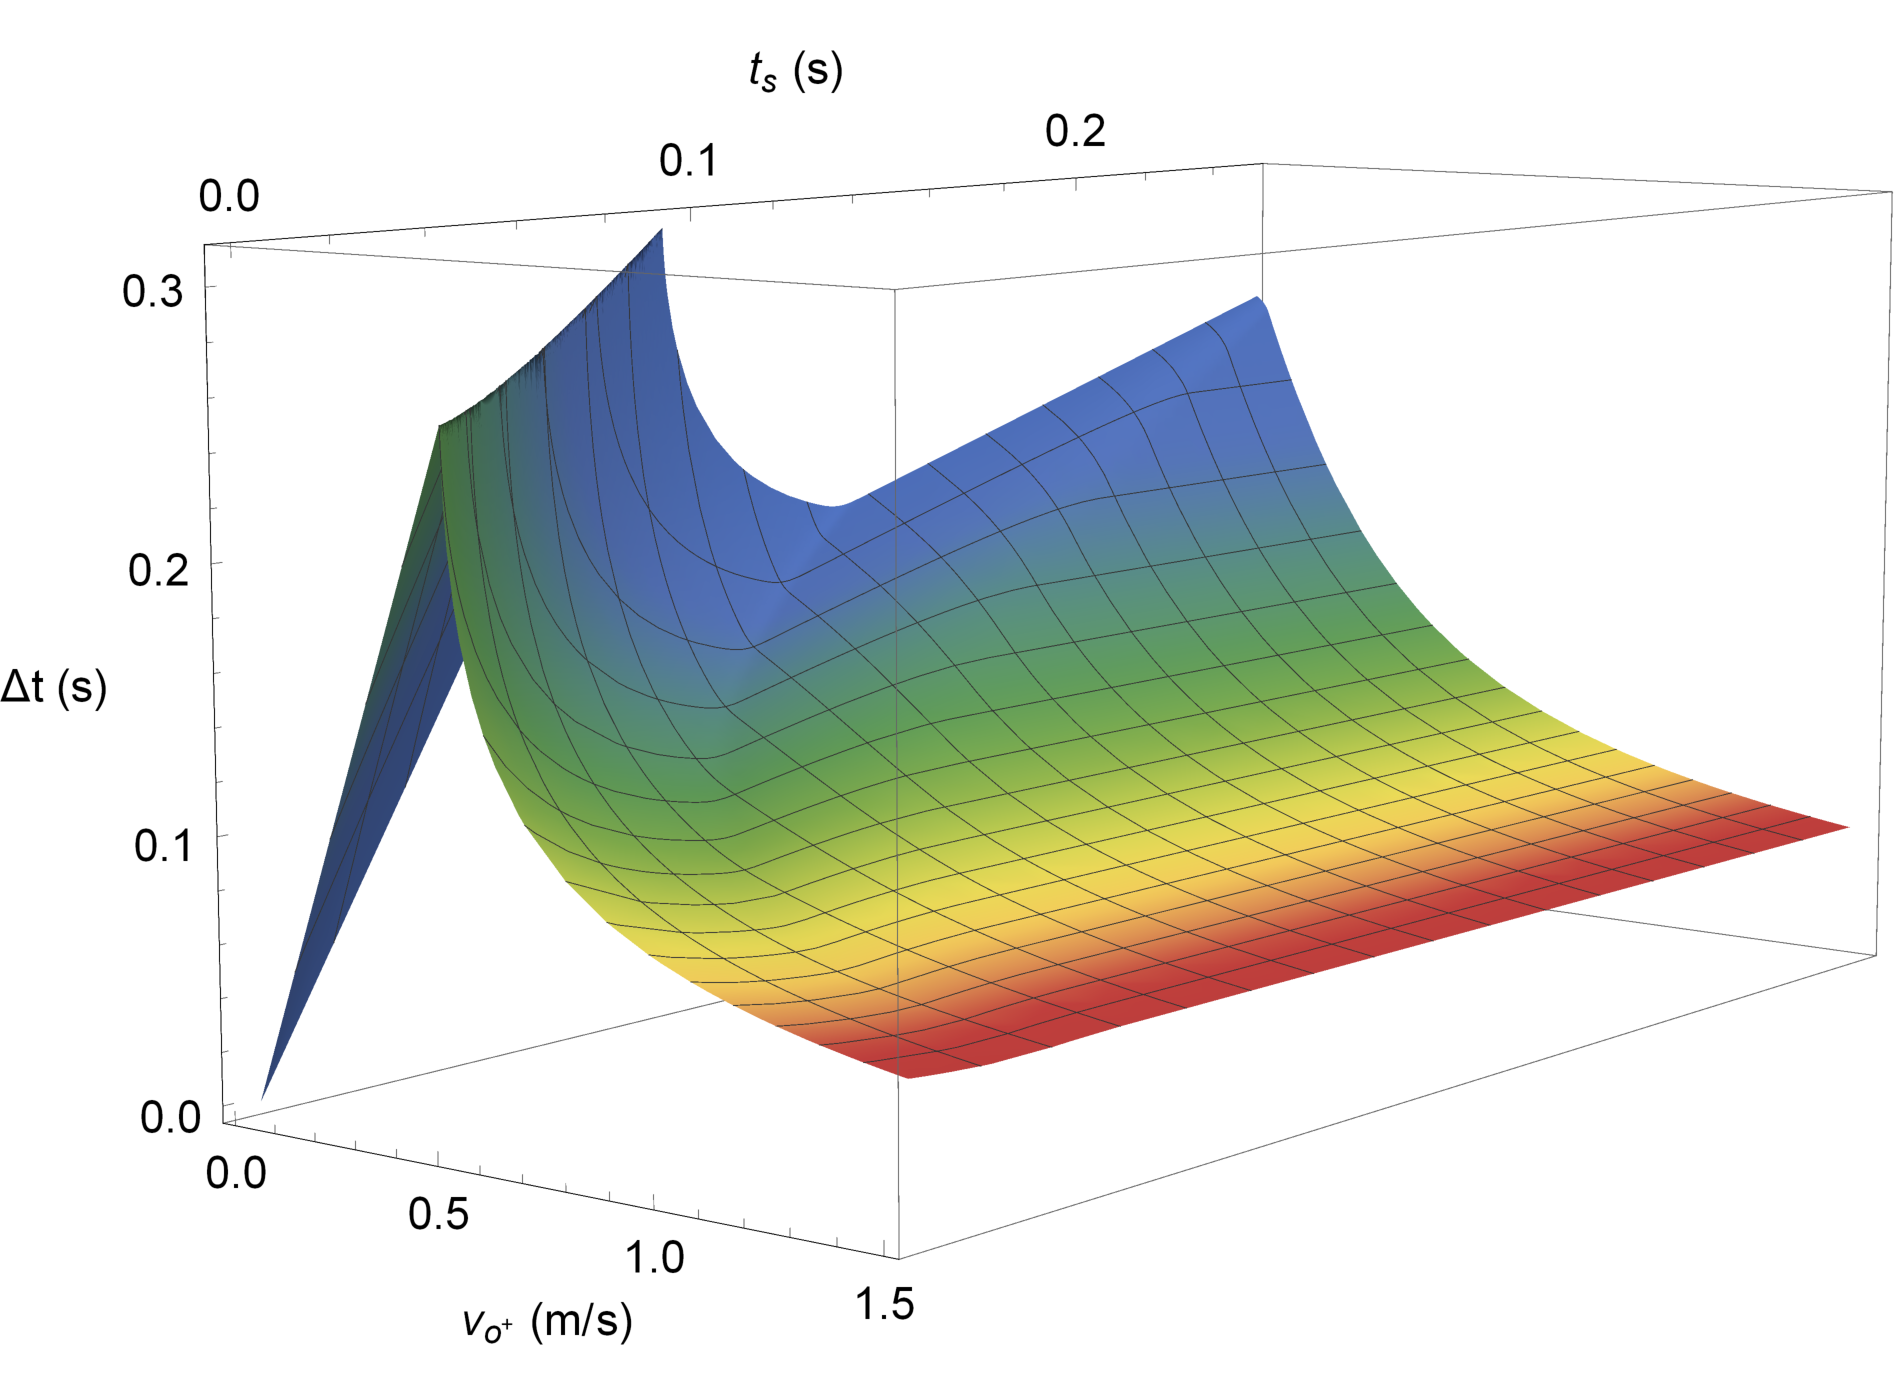
\includegraphics[width=\linewidth]{3Dcontour_view1.pdf}
	\caption[3D contour plot of time between impacts vs. switching time vs. initial velocity - 1]{3D contour plot of $\Delta t$ vs. $t_s$ plotted for different values of $v_{o+}$.   $t_s$ is a control parameter and $\Delta t$ can be obtained by sensing.  Together, $\Delta t$ and $t_s$ can be used to estimate $v_{o+}$ with our estimator.}
	\label{3Dcontour}
\end{figure}

\subsubsection{Effect of Coulomb friction}
\label{frictionwriteup}
\begin{figure}
	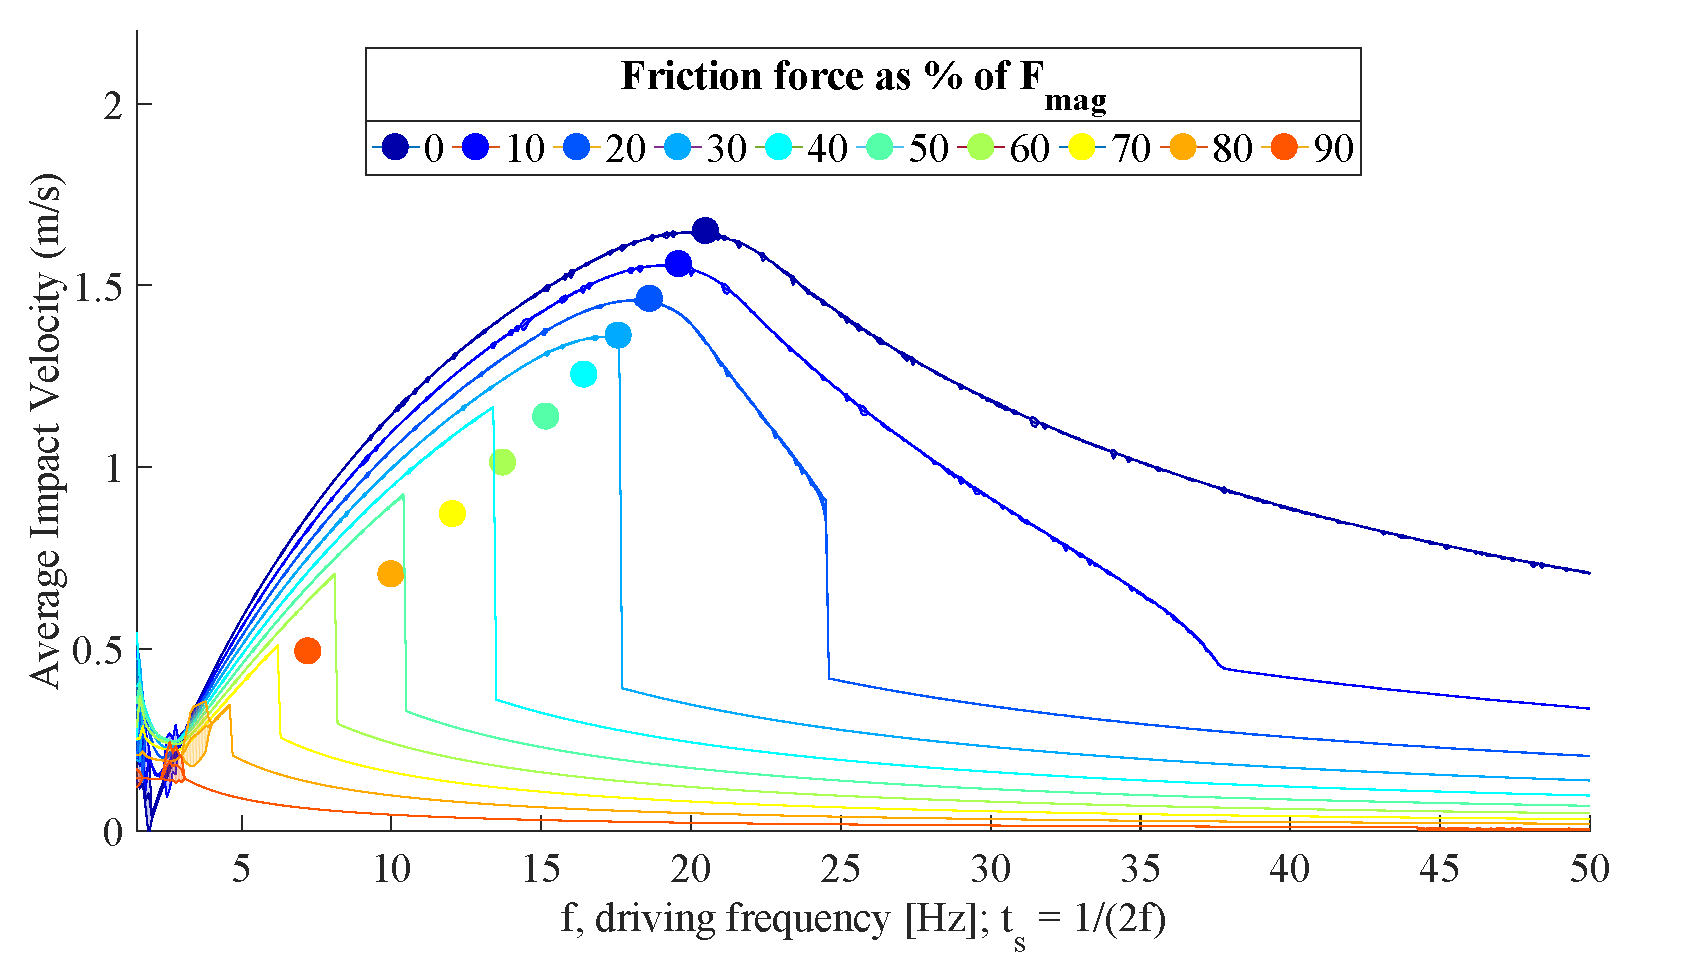
\includegraphics[width=\linewidth]{FrictionForceWithClosedLoopValues.pdf}
		\caption[Effect of Coulomb friction on partially closed-loop control]{Comparison of  simulated impact velocities. The  velocities for impacts 100 to 200 are averaged and plotted for different values of Coulomb friction force. Colored circles represent the ideal closed-loop values.  Lines represent the partially closed-loop values.}
	\label{friction}
	
\end{figure}
In all the above models, the friction force was assumed to be zero. Average impact velocities over 100 impacts are plotted for varying values of the friction force in Fig. \ref{friction}. The circles represent the ideally-closed loop values, while the curves represent the partially closed-loop values using impact times. Much like the step-out frequency of a stepper motor, average impact velocities drop suddenly for the partially closed-loop system beyond a cut-off driving frequency. This is due to the sphere reversing direction before spring contact, leading to a drop in its net kinetic energy. As friction force increases as a percentage of $F_{mag}$, the partially closed loop system reaches its cutoff frequency, before resonance. This drop in impact velocity is not seen in the fully closed-loop system, for any values of friction. Hence, partially closed-loop control will not produce the maximum possible impact velocity for high values of Coulomb friction force. 


\section{Experimental determination of Impact coefficient of resititution}
\label{cor_det}
The coefficient of restitution $e$ was determined using the time interval between two consecutive bounces of the sphere when dropped from a given height onto the impact rod. The measurements were made using 38.1 mm long impact rods for five different materials. Impact rods were held by a drill chuck. A length of 10.0 mm of the impact rods was sticking out of the chuck. The experimental setup is shown in \cref{CoR_setup_data}.

The results, shown in fig. \ref{CoR_Results}, show that and that aluminum offers the largest coefficient of restitution, followed by titanium and brass. The densities of aluminum, titanium, stainless steel, brass, and copper are 2720, 4500, 7600, 8500, and 8940 kg/m$^3$ respectively. This data, coupled with a desire for a lightweight millirobot suggests that titanium is the best material for an impact plate. Bio-compatibility of the material used is another constraint.

\begin{figure}
	\includegraphics[width=\columnwidth]{CoR_setup_data.eps}
	\caption{Experimental setup for measuring the coefficient of restitution $e$}
	\label{CoR_setup_data}
\end{figure}

\begin{figure}
	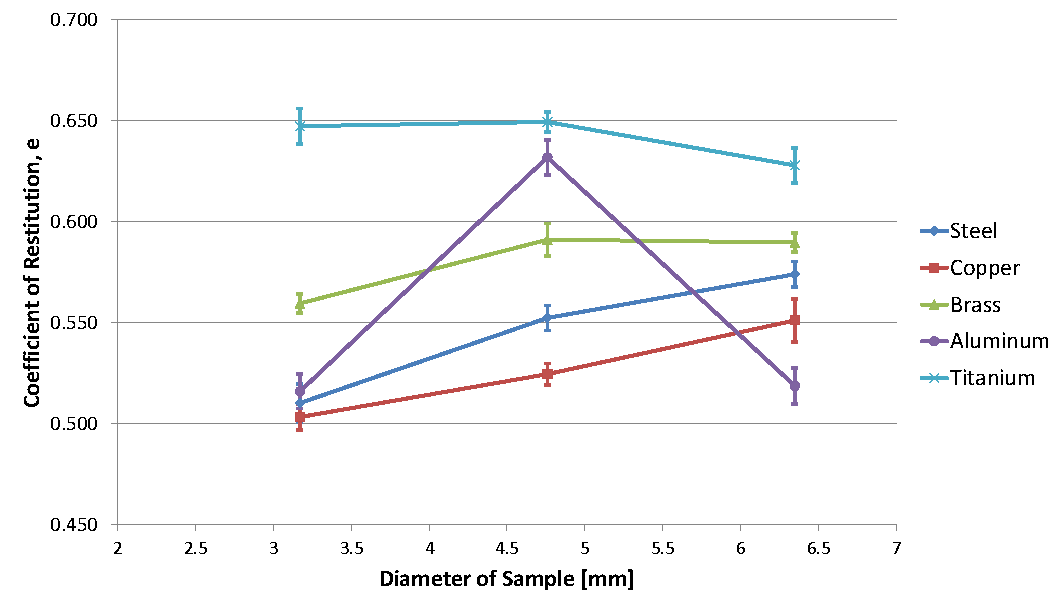
\includegraphics[width=\columnwidth]{CoRdata.pdf}
	\caption[Comparison of measured coefficients of restitution for different materials]{Measured coefficient of restitution $e$ as a function of rod diameter for different materials}
	\label{CoR_Results}
\end{figure}





\section{Experimental magnetic hammer tests}
\label{experiment}
\subsection{Magnetic test bench description}

A desktop-size, single-axis magnetic setup was built to reduce the cost related to clinical MRI experiments.
 It is composed of two solenoid coils oriented along the same axis and separated by a distance $d$. 
 The coils are used to produce both the magnetizing field and the gradient. 
 The properties of the coils are shown in Table \ref{coil_table}.\par
The system is shown in \cref{magnetic_setup}.
 The two coils are held by an acrylic tube. 
 They can slide along this tube and be locked in place to adjust the distance between the two coils and therefore change the maximum field and gradient values. 
 The acrylic tube is transparent, allowing for visual access to the robot.
Each coil is powered via a Syren 25 switch mode power supply. 
A Hall-effect-based current sensor is used to perform a PID regulation of the current. 
It is necessary to control the current inside the coils and not only the voltage. 
Indeed, the produced magnetic field is directly proportional to the current whereas the voltage is related to the magnetic flux variation and the voltage drop produced by Joule effect losses.\par
Robots are inserted inside the acrylic tube holding the coils. 
They are held by a second, smaller tube that guides them along the system axis. 
Robots can be free to move along the coil axis or held in place. 
A picture of the system is provided in \cref{magnetic_setup}.

\begin{figure}
  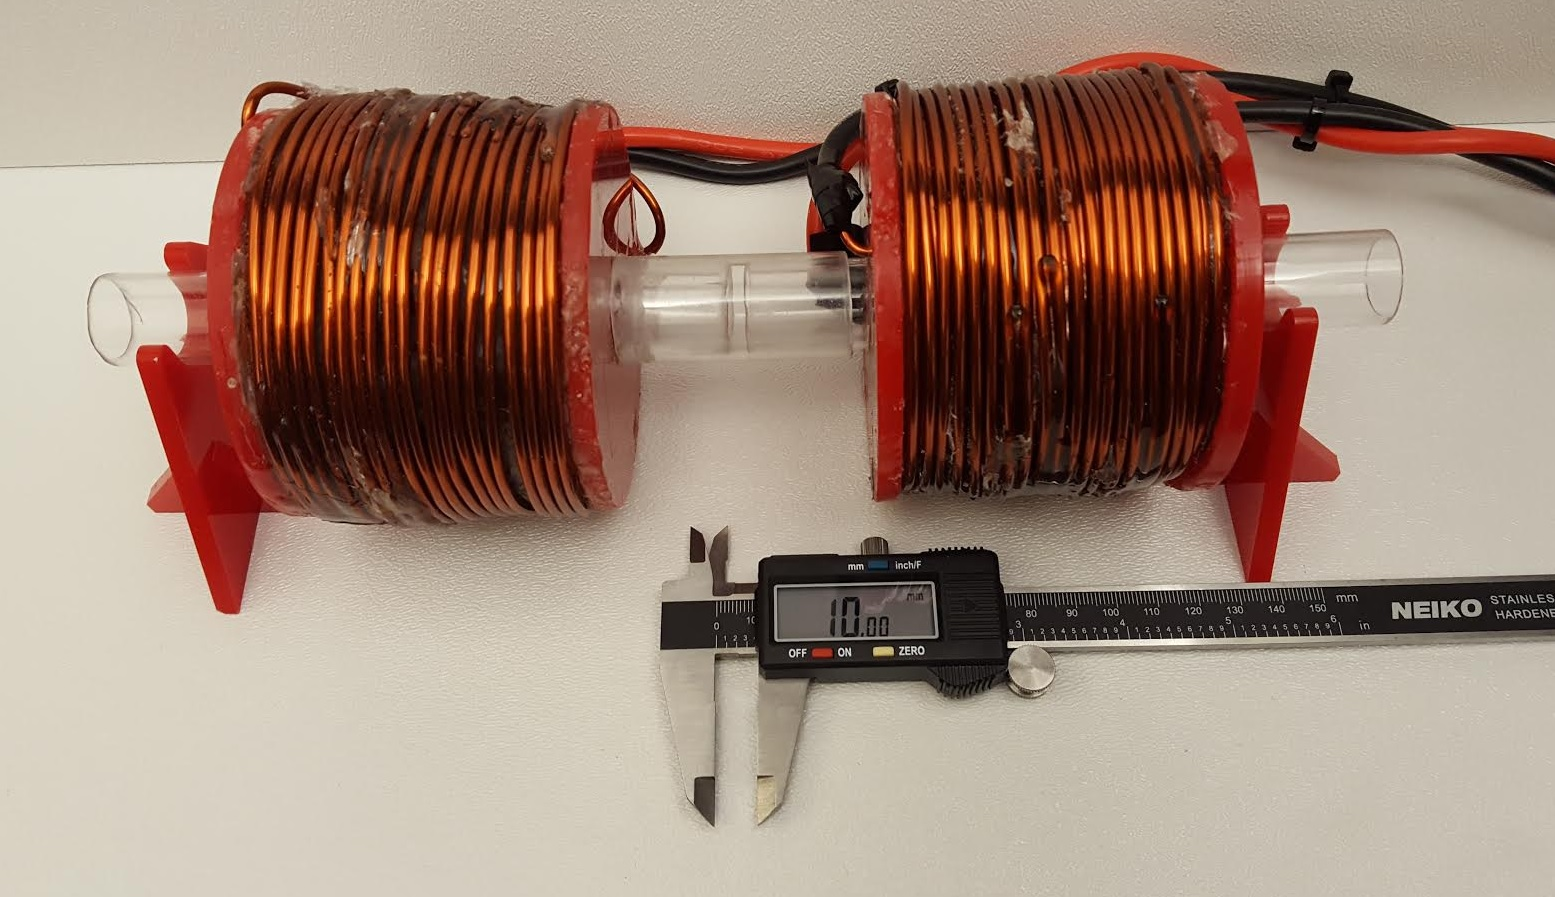
\includegraphics[width=\linewidth]{Magnetic_setup.jpg}
  \caption{Picture of the desktop-size magnetic setup.}
  \label{magnetic_setup}
\end{figure}

\begin{table}[]
\centering
\caption{Properties of the coils used in the desktop-size test bench}
\label{coil_table}
\begin{tabular}{|l|l||l|l|}
\hline
Internal Radius    & 12.7 mm                   & Electrical resistance                                                                      & 0.16 $\Omega$       \\ \hline
External Radius    & 45.8 mm                   & Inductance                                                                                 & 1.59 mH    \\ \hline
Length             & 65 mm                     & \begin{tabular}[c]{@{}l@{}}Max current change rate \\ Voltage = 25 V\end{tabular}          & 15.7 kA/s \\ \hline
Wire               & 10 AWG                    & Max continuous current                                                                 & 15 A       \\ \hline
Wire cross-section & 5.26 mm$^2$ & \begin{tabular}[c]{@{}l@{}}Flux density on \\ system center\\ I = 15 A, $d$ = 50 mm\end{tabular} & 11 mT      \\ \hline
Number of turns    & 265                       & \begin{tabular}[c]{@{}l@{}}Gradient on \\system center\\  I = 15 A, $d$ = 50 mm\end{tabular}    & 0.45 T/m   \\ \hline
\end{tabular}
\end{table}


\subsection{Partially closed loop experiment}

The coils are driven by square shaped current waveform. 
The current in the coils can either be $I_{max}$ or 0 A. 
The coil will be said to be ``on'' when $I=I_{max}$ and ``off'' when $I=0$ A.\par
As explained in \cref{clol}, the magnetic hammer cannot work properly if the magnetic field is not synchronized with the position of the sphere.
 An open-loop control is inefficient, as shown in Fig.~\ref{CLvsOL}.
  The force applied on the sphere (and therefore the magnetic gradient) must change direction when the sphere hits the impact plate and when the sphere changes direction on the spring side to provide maximum impulse.\par
Our eventual goal is to use these robots in an MRI scanner, where MRI gradients must be shared for propulsion and position feedback \cite{578}. 
The nature of our system enables simpler sensing requirements that can be accomplished with a simple microphone. 
The microphone is used to monitor the noise produced by the system. 
The impact noise creates a larger pulsed signal on the microphone output and can, therefore, be easily detected. 
When the impact is detected, the anterior coil is turned off while the posterior coil is turned on. 
The force applied on the sphere now pushes it backward, toward the spring side.\par
The current stays constant during a time $T_s$ after the impact is detected. 
The anterior coil is subsequently turned on, and the posterior coil is turned off. 
The force then pushes the sphere forward. The current in the coils is changed again when another impact is detected. 
This process is repeated indefinitely.\par
$T_s$ is manually tuned while the system is working. 
It is set to the value that gives the maximum oscillating frequency. 
This value corresponds to a gradient that changes direction when the sphere velocity is zero on the spring side. 
It should give the same results as the perfectly closed-loop simulations.\par
The partially closed-loop experiment was performed and compared to the model. 
Section \ref{experiment} shows a comparison of the optimum oscillating frequency as a function of $I_{max}$. 
The simulations are performed for a perfectly-closed loop system. 
When $I_{max}$ increases, the oscillating frequency increases. 
The force on the sphere  increases with $I_{max}$ and consequently increases the moving speed of the sphere.
This figure also shows that the model without friction has the same slope as the experimental data. 
However, the simulation signals are approximately 1 Hz faster than the experiment. 
This difference probably comes from the lack of friction in the model. 
The next subsection adds the effect of friction to the model.

\begin{figure}
  \includegraphics[width=\linewidth]{figure3.eps}
  \caption{Comparison between the oscillating frequency obtained experimentally and with the model as a function of the current in the coils $I_{max}$.}
  \label{freq}
\end{figure}

\subsection{Effect of friction}

To improve the model accuracy, the friction between the moving sphere and the other components of the millirobot was included into the model. 
The sphere can be rolling or sliding inside the tube. 
The modelization is based on the method described in \cite{00319120303009}. 

The rotation speed $\dot{\theta} $ is first computed and drag is calculated from this result.\par

The friction on the tube produces a torque on the sphere. 
It is assumed that the coefficient of static friction is equal to the coefficient of kinetic friction $\mu_k$. 
The equation used to calculate the angular velocity variation $\frac{\mathrm{d\dot{\theta} } }{\mathrm{d} t}$ of the sphere is different whether the sphere is rolling or sliding. 
The distinction between this two different behavior is made by calculating the relative velocities $V_{rel}$ of the sphere and the tube surface (see \cref{relV}). \par


\begin{equation}
V_{rel}=V-r\dot{\theta}
\label{relV}
\end{equation}

 
If the relative speed is inferior to 0.005 m/s and if the force applied to the sphere is smaller than the kinetic friction, the sphere is considered to be rolling inside the tube and the drag is null. $\frac{\mathrm{d\dot{\theta} } }{\mathrm{d} t}$ can be calculated with:

\begin{equation}
\frac{\mathrm{d\dot{\theta} } }{\mathrm{d} t}=r\frac{\mathrm{dV } }{\mathrm{d} t}
\label{domega}
\end{equation}

In all other cases, the torque applied to the sphere is equal to the kinetic friction force multiplied by the sphere radius. The drag is equal to the kinetic friction force $\mu_k$ = 0.2.\par
Results of simulations are shown in Fig. \ref{freq}. The addition of the friction greatly improves the model accuracy.

%\section{Tissue penetration test}
%\begin{table}[h]
%\caption{An Example of a Table}
%\label{table_example}
%\begin{center}
%\begin{tabular}{|c||c|}
%\hline
%One & Two\\
%\hline
%Three & Four\\
%\hline
%\end{tabular}
%\end{center}
%\end{table}


%   \begin{figure}[thpb]
%      \centering
%      \framebox{\parbox{3in}{We suggest that you use a text box to insert a graphic (which is ideally a 300 dpi TIFF or EPS file, with all fonts embedded) because, in an document, this method is somewhat more stable than directly inserting a picture.
%}}
%      %\includegraphics[scale=1.0]{figurefile}
%      \caption{Inductance of oscillation winding on amorphous
 %      magnetic core versus DC bias magnetic field}
 %     \label{figurelabel}
 %  \end{figure}
\section{Preliminary tests in clinical mri}
\label{MRI_tests}
Preliminary tests of magnetic hammers were performed in a clinical 3T Siemens MRI scanner. 
No closed-loop control was implemented. 
The magnetic gradient  oscillated at a constant frequency. 
As seen before, the system does not work optimally in these conditions. 
At low frequencies, the ferromagnetic sphere completely stops on both sides of the millirobot. 
All the kinetic energy is lost at these times, and the magnetic hammer, therefore, performs poorly. 
The aim of this tests is to prove that MRI scanners are suitable to produce the desired force on the magnetic sphere inside the millirobot and provide a pulsed force.\par
A 50 mm long, 7 mm diameter robot was built for this test. 
A 2Hz square gradient with an amplitude of 23 mT/m was applied to it. 
This frequency is slow enough to allow the sphere to stop on both sides completely. 
A sheep brain hemisphere was used as tissue sample to penetrate.\par
Once the gradient wave was started, the sphere began to move back and forth while the robot was moving toward the sample at each impact, at an average speed of 1.9 mm/s. Friction with the plastic container prevent the capsule from moving if a constant gradient is applied. 
 The robot then began to penetrate the sample. It went 9 mm deep inside it and stopped progressing (see \cref{MRI_test}). 
This experiment demonstrated the suitability of MRI scanner to drive magnetic hammers. \par
Future work will implement closed loop control on the clinical MRI scanner to transfer energy efficiently. 
The MRI signal could be used to compute the position of the magnetic sphere at a frequency greater than 20 Hz, as we did in~\cite{578}.

\begin{figure}
\centering
  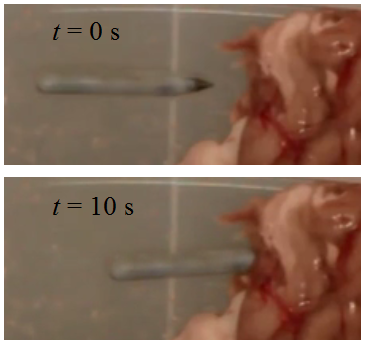
\includegraphics[width=150 pt]{tests_in_MRI.png}
  \caption{Picture of the magnetic hammer driven by an MRI scanner. The penetration test is realized on a sheep brain sample.}
  \label{MRI_test}
\end{figure}

\section{CONCLUSIONS}
\label{conclusion}
A magnetic hammer system for a millirobot driven by the gradient fields of an MRI scanner was studied. 
The system enables producing the forces large enough to penetrate body tissue.\par
The hammer is composed of a ferromagnetic sphere moving inside a tube. 
On the posterior side of the robot, there is a spring that allows changing the direction of the sphere smoothly. 
On the anterior side, a hard metal rod act as an impact plate to transfer the momentum of the ferromagnetic sphere to the body of the robot.\par
The system is driven by an external magnetic field, such as that produced by an MRI scanner. 
The main field magnetizes the sphere and the gradient produces the forces necessary to move the sphere.\par
 A complex modelization allows the computation of the position of the sphere as a function of time. 
 The magnetic flux density and the gradient are computed using a semi-analytical method and allow an accurate calculation of the force applied to the sphere. 
 The speed of the sphere after impact is computed from the coefficient of restitution. 
 The rotation of the sphere is also calculated, allowing an accurate calculation of the drag produced by the sliding of the sphere inside the tube.\par

The coefficients of restitution ($e$) depends on the materials of the colliding objects but also on their shape and sizes. 
Values of $e$ were experimentally measured. 
These measurements showed that aluminum impact plates exhibit large values of $e$. 
This material also has the advantage of being lightweight, a useful property to achieve neutral buoyancy of millirobots. 
Titanium also performs well, is lightweight and is a bio-compatible material.\par

A desktop-size magnetic test bench was built to reduce experimental cost related to the use of a clinical MRI scanner. 
A magnetic hammer was tested with a partially closed loop control. 
The impact of the sphere is detected via a microphone. 
The posterior coil is turn on during a predetermined time to pull the sphere backward.
 After this time, the posterior coil is turned off and the anterior coil is turned on until the next impact is detected. 
 Experimental results were compared to the model.
  The experimental oscillating frequency is in good agreement with the model predictions. 
  This validates our modelization.\par
In future work, the control of the magnetic hammer will be implemented and tested in a clinical MRI scanner. 
The impact will be detected with the MRI signal instead of a microphone. 
The tradeoffs involved in miniaturization of the robot will also be studied.

 

\addtolength{\textheight}{-12cm}   % This command serves to balance the column lengths
                                  % on the last page of the document manually. It shortens
                                  % the textheight of the last page by a suitable amount.
                                  % This command does not take effect until the next page
                                  % so it should come on the page before the last. Make
                                  % sure that you do not shorten the textheight too much.

%%%%%%%%%%%%%%%%%%%%%%%%%%%%%%%%%%%%%%%%%%%%%%%%%%%%%%%%%%%%%%%%%%%%%%%%%%%%%%%%



%%%%%%%%%%%%%%%%%%%%%%%%%%%%%%%%%%%%%%%%%%%%%%%%%%%%%%%%%%%%%%%%%%%%%%%%%%%%%%%%

\bibliographystyle{unsrt}
\bibliography{biblio}



\end{document}
